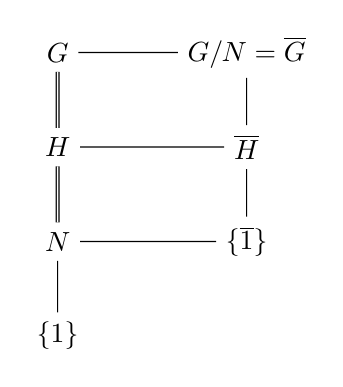
\begin{tikzpicture}[scale=1.2]
  % Nodes
  \node (G) at (-1,3) {$G$};
  \node (G/N) at (1,3) {$G/N=\overline{G}$};
  \node (H) at (-1,2) {$H$};
  \node (Hb) at (1,2) {$\overline{H}$};
  \node (N) at (-1,1) {$N$};
  \node (1b) at (1,1) {$\{\overline{1}\}$};
  \node (1) at (-1,0) {$\{1\}$};

  % Lineas nodos
  \draw[double] (G) -- (H);
  \draw[double] (H) -- (N);
  \draw (G) -- (G/N);
  \draw (G/N) -- (Hb);
  \draw (H) -- (Hb);
  \draw (Hb) -- (1b);
  \draw (N) -- (1b);
  \draw (N) -- (1);
\end{tikzpicture}
